There are several visualization tools that can be used for \amrex\
plotfiles.  The standard tool used within the
\amrex-community is \amrvis, a package developed and supported 
by CCSE that is designed specifically for highly efficient visualization
of block-structured hierarchical AMR data.
Plotfiles can also be viewed using the \visit, \paraview, and \yt packages.
Particle data can be viewed using \paraview.

\section{\amrvis}

Our favorite visualization tool is \amrvis. We heartily encourage you
to build the {\tt amrvis2d} and {\tt amrvis3d} executables, and to try using them
to visualize your data. A very useful feature is View/Dataset, which
allows you to actually view the numbers in a spreadsheet that is nested
to reflect the AMR hierarchy -- this can be handy for
debugging. You can modify how many levels of data you want to see,
whether you want to see the grid boxes or not, what palette you use,
etc.  Here are some instructions and tips for using \amrvis:

\begin{enumerate}

\item Download and build \amrvis:
\begin{verbatim}
git clone https://ccse.lbl.gov/pub/Downloads/Amrvis.git
\end{verbatim}

Then {\tt cd} into {\tt Amrvis/}, edit the {\tt GNUmakefile} by
setting {\tt COMP} to the compiler suite you have.

Type {\tt make DIM=2} or {\tt make DIM=3} to build, 
resulting in an executable that looks like {\tt amrvis2d...ex}.

If you want to build amrvis with {\tt DIM=3}, you must first
download and build {\tt volpack}:
\begin{verbatim}
git clone https://ccse.lbl.gov/pub/Downloads/volpack.git
\end{verbatim}

Then {\tt cd} into {\tt volpack/} and type {\tt make}.

Note: \amrvis\ requires the OSF/Motif libraries and headers. If you don't have these 
you will need to install the development version of motif through your package manager. 
{\tt lesstif} gives some functionality and will allow you to build the amrvis executable, 
but \amrvis\ may exhibit subtle anomalies.

On most Linux distributions, the motif library is provided by the
{\tt openmotif} package, and its header files (like {\tt Xm.h}) are provided
by {\tt openmotif-devel}. If those packages are not installed, then use the
OS-specific package management tool to install them. 

You may then want to create an alias to {\tt amrvis2d}, for example
\begin{verbatim}
alias amrvis2d /tmp/Amrvis/amrvis2d...ex
\end{verbatim}

\item Run the command {\tt cp Amrvis/amrvis.defaults \textasciitilde/.amrvis.defaults}.
Then, in your copy, edit the line containing ``{\tt palette}'' line to point to, e.g., 
``{\tt palette  /home/username/Amrvis/Palette}''.  The other lines control
options such as the initial field to display, the number format, widow size, etc.
If there are multiple instances of the same option, the last option takes precedence.

\item Generally the plotfiles have the form {\tt pltXXXXX} 
  (the {\tt plt} prefix can be changed), where {\tt XXXXX} is a number 
  corresponding to the timestep the file
  was output.  {\tt amrvis2d <filename>} or {\tt amrvis3d <filename>}
  to see a single plotfile, 
  or for 2D data sets, {\tt amrvis2d -a plt*}, which will animate the 
  sequence of plotfiles.

  You can use the ``Variable'' menu to change the variable.
  You can left-click drag a box around a region
  and click "View'' $\rightarrow$ ``Dataset''
  in order to look at the actual numerical values
  (see Figure \ref{Fig:Amrvis}).
  Or you can simply left click on a point to obtain the numerical value.
  You can also export the
  pictures in several different formats under "File/Export".
  In 2D you can right and center click to get line-out plots.
  In 3D you can right and center click to change the planes, and the hold
  shift+(right or center) click to get line-out plots.

\begin{figure}[tb]
\centering
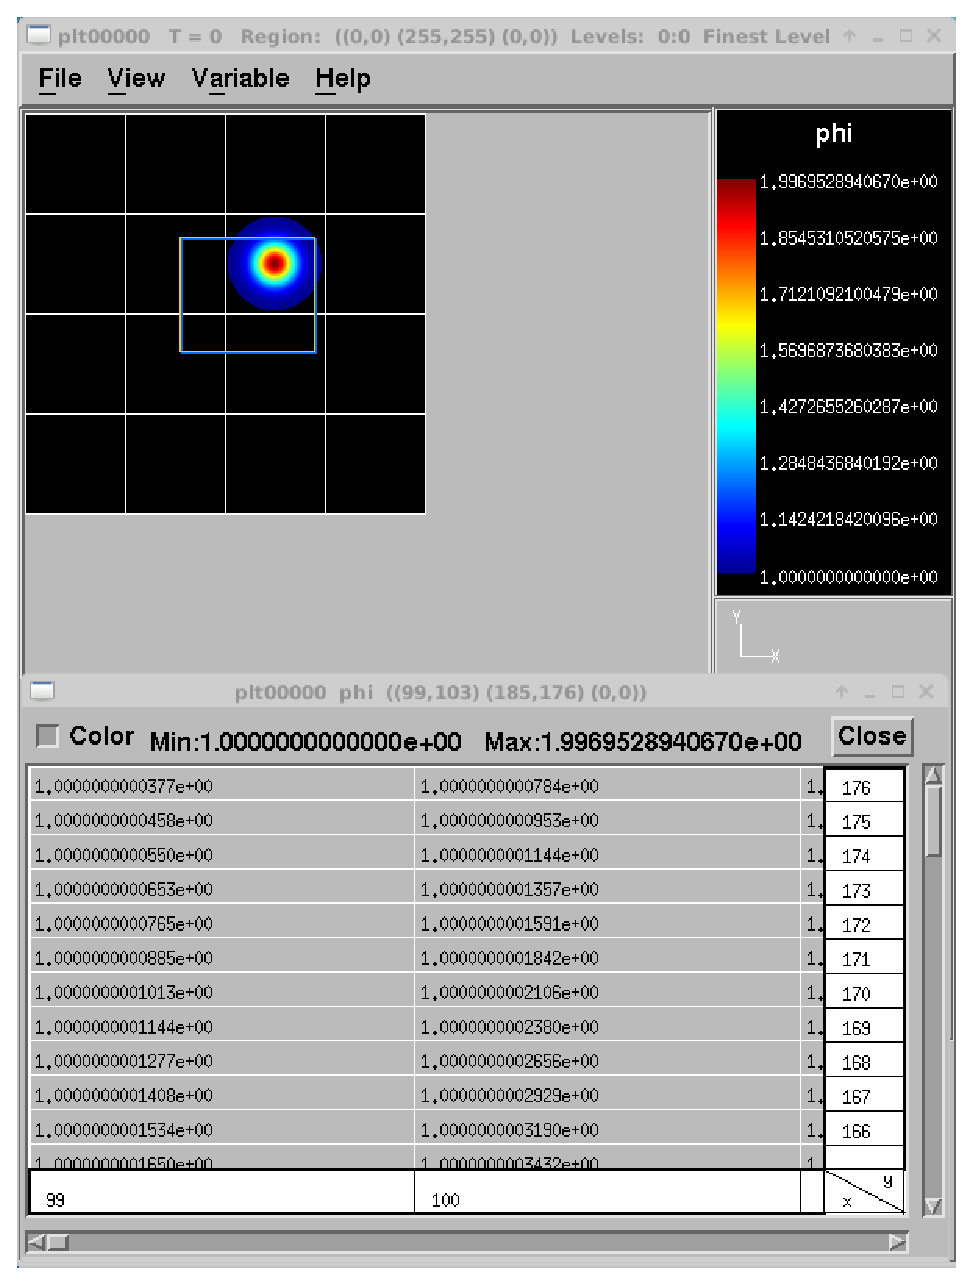
\includegraphics[width=2.5in]{./Visualization/Amrvis_2d}
~~~
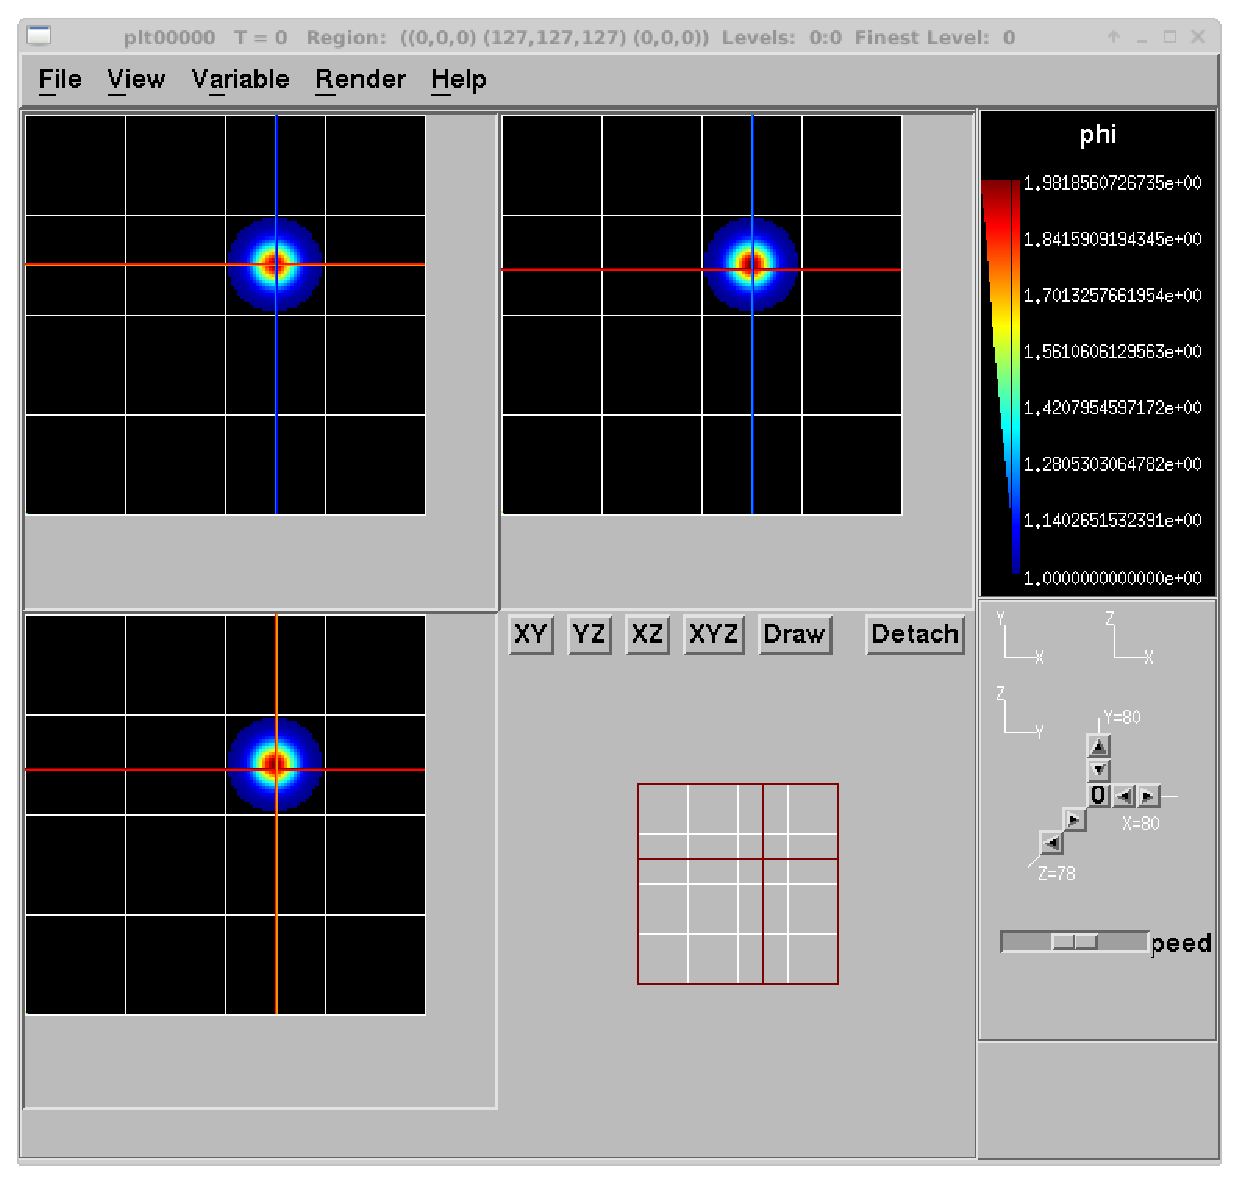
\includegraphics[width=2.5in]{./Visualization/Amrvis_3d}
\caption{2D and 3D images generated with Amrvis}
\label{Fig:Amrvis}
\end{figure}

  We have created a number of routines to convert \amrex\ plotfile data
  other formats (such as MATLAB), but in order to properly interpret 
  the hierarchical AMR data, each tends to have its own idiosyncrasies.
  If you would like to display the data in another format, please contact
  Marc Day ({\tt MSDay@lbl.gov}) and we will point you to whatever we have
  that can help.

\end{enumerate}

\section{\visit}
\label{sec:visit}

\amrex\ data can also be visualized by {\tt VisIt}, an open
source visualization and analysis software.  To follow along with this example,
first build and run the first heat equation tutorial code
(see Section \ref{sec:heat equation}).

Next, download and install {\tt VisIt} from \url{https://wci.llnl.gov/simulation/computer-codes/visit}.
To open a single plotfile, run {\tt VisIt}, then select ``File'' $\rightarrow$ ``Open file ...'',
then select the {\tt Header} file associated the the plotfile of interest (e.g., {\tt plt00000/Header}).
Assuming you ran the simulation in 2D, here are instructions for making a simple plot:
\begin{itemize}
\item To view the data, select ``Add'' $\rightarrow$ ``Pseudocolor'' $\rightarrow$ ``phi'', and then select
``Draw''.
\item To view the grid structure (not particularly interesting yet, but when we add AMR it will be), select
`` $\rightarrow$ ``subset'' $\rightarrow$ ``levels''.  Then double-click the text ``Subset - levels'',
enable the ``Wireframe'' option, select ``Apply'', select ``Dismiss'', and then select ``Draw''.
\item To save the image, select ``File'' $\rightarrow$ ``Set save options'', then customize the image format
to your liking, then click ``Save''.
\end{itemize}
Your image should look similar to the left side of Figure \ref{Fig:VisIt}.\\
\begin{figure}[tb]
\centering
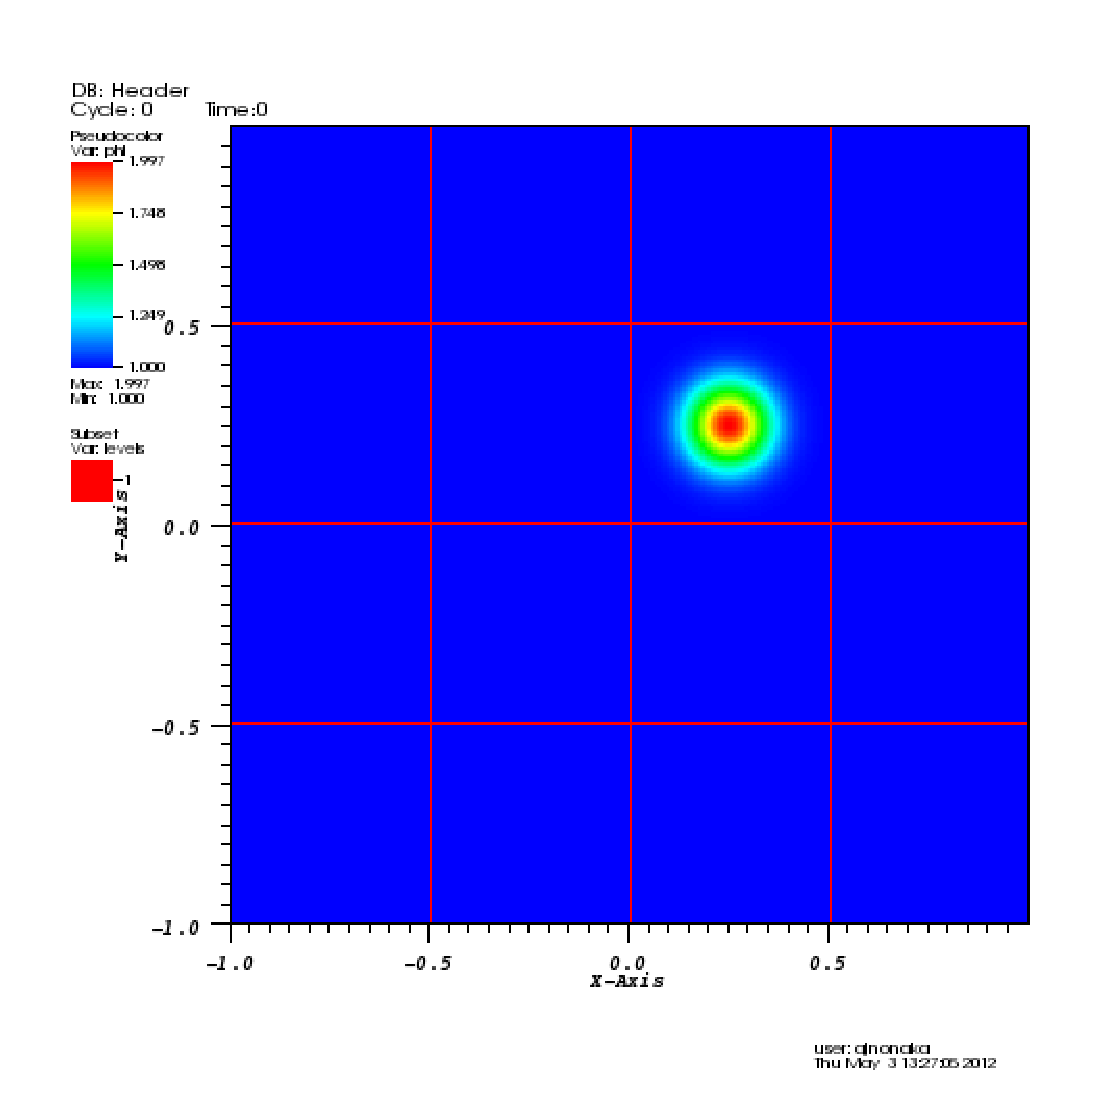
\includegraphics[width=3.1in]{./Visualization/VisIt_2D}
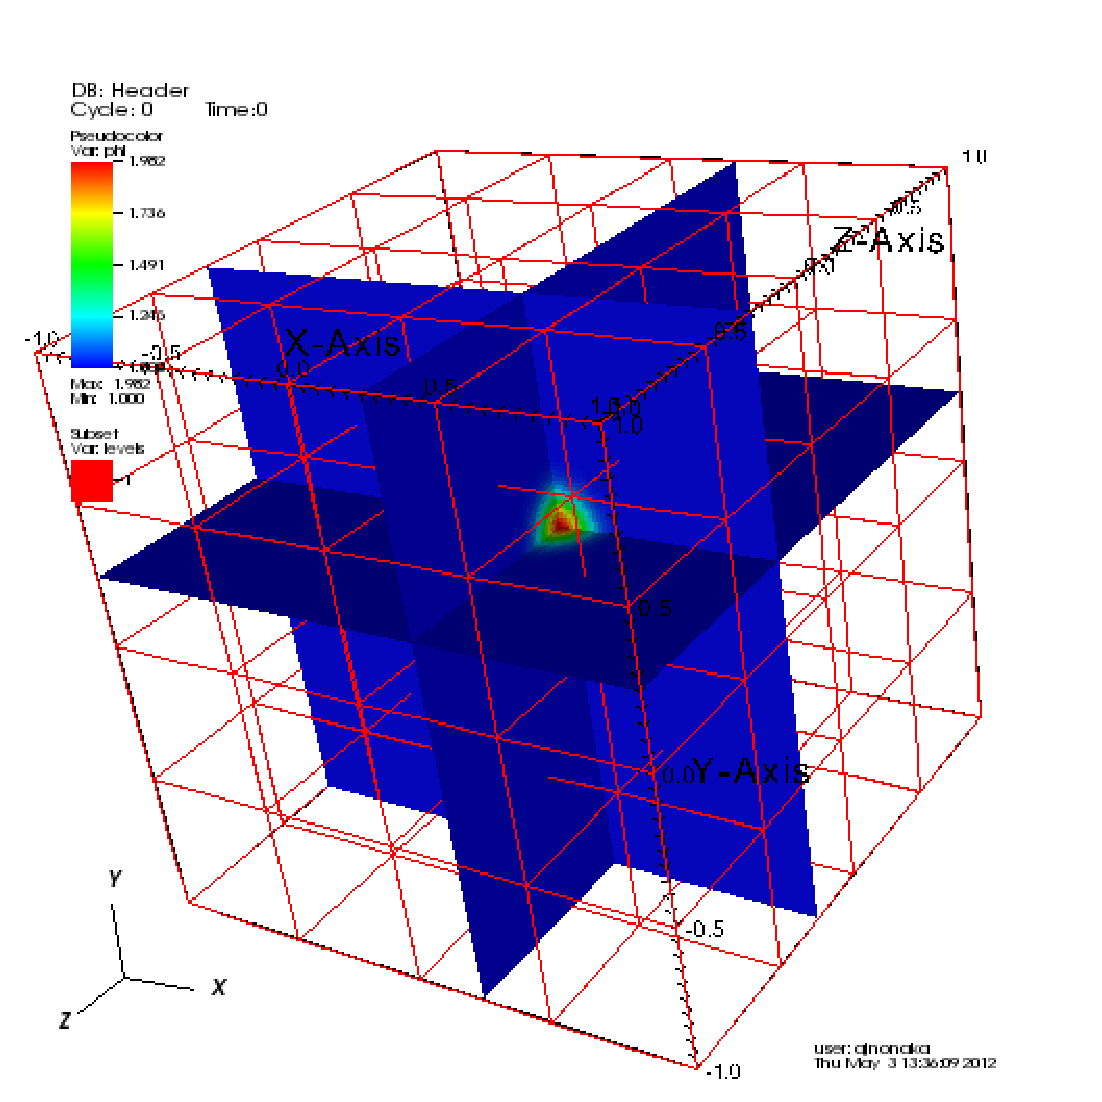
\includegraphics[width=3.1in]{./Visualization/VisIt_3D}
\caption{(Left) 2D image generated with VisIt.  (Right) 3D image generated with VisIt.}
\label{Fig:VisIt}
\end{figure}

In 3D, you must apply the ``Operators'' $\rightarrow$ ``Slicing'' $\rightarrow$ ``ThreeSlice'', with the 
``ThreeSlice operator attribute'' set to x=0.25, y=0.25, and z=0.25.  You can left-click and drag
over the image to rotate the image to generate something similar to right side of Figure \ref{Fig:VisIt}.\\

To make a movie, you must first create a text file named {\tt movie.visit} with a list of the {\tt Header} 
files for the individual frames.  This can most easily be done using the command:
\begin{lstlisting}[backgroundcolor=\color{light-red}]
~/amrex/Tutorials/Basic/HeatEquation_EX1_C> ls -1 plt*/Header | tee movie.visit
plt00000/Header
plt01000/Header
plt02000/Header
plt03000/Header
plt04000/Header
plt05000/Header
plt06000/Header
plt07000/Header
plt08000/Header
plt09000/Header
plt10000/Header
\end{lstlisting}
The next step is to run {\tt VisIt}, select ``File'' $\rightarrow$ ``Open file ...'',
then select {\tt movie.visit}.  Create an image to your liking and press the ``play'' button
on the VCR-like control panel to preview all the frames.  To save the movie, choose
``File'' $\rightarrow$ ``Save movie ...'', and follow the on-screen instructions.

\section{\paraview}
The open source visualization package \paraview\ v5.3.0 can be used to view 
3D plotfiles, and v5.4.0 can be used to view particle data.  Download
the package at \url{https://www.paraview.org/}.  

To open a single plotfile (for example, you could run the {\tt HeatEquation\_EX1\_C} in 3D:
\begin{enumerate}
\item Run \paraview\ v5.3.0, then select ``File'' $\rightarrow$ ``Open''.
\item Navigate to the plotfile directory, and manually type in ``Header''.
      \paraview\ will ask you about the file type -- choose ``Boxlib 3D Files''
\item Under the ``Cell Arrays'' field, select a variable (e.g., ``phi'') 
      and click ``Apply''.
\item Under ``Representation'' select ``Surface''.
\item Under ``Coloring'' select the variable you chose above.
\item To add planes, near the top left you will see a cube icon with a green plane
      slicing through it.  If you hover your mouse over it, it will say ``Slice''.
      Click that button.
\item You can play with the Plane Parameters to define a plane of data to view, as shown
      in Figure \ref{fig:ParaView}.
\end{enumerate}

\begin{figure}[tb]
\centering
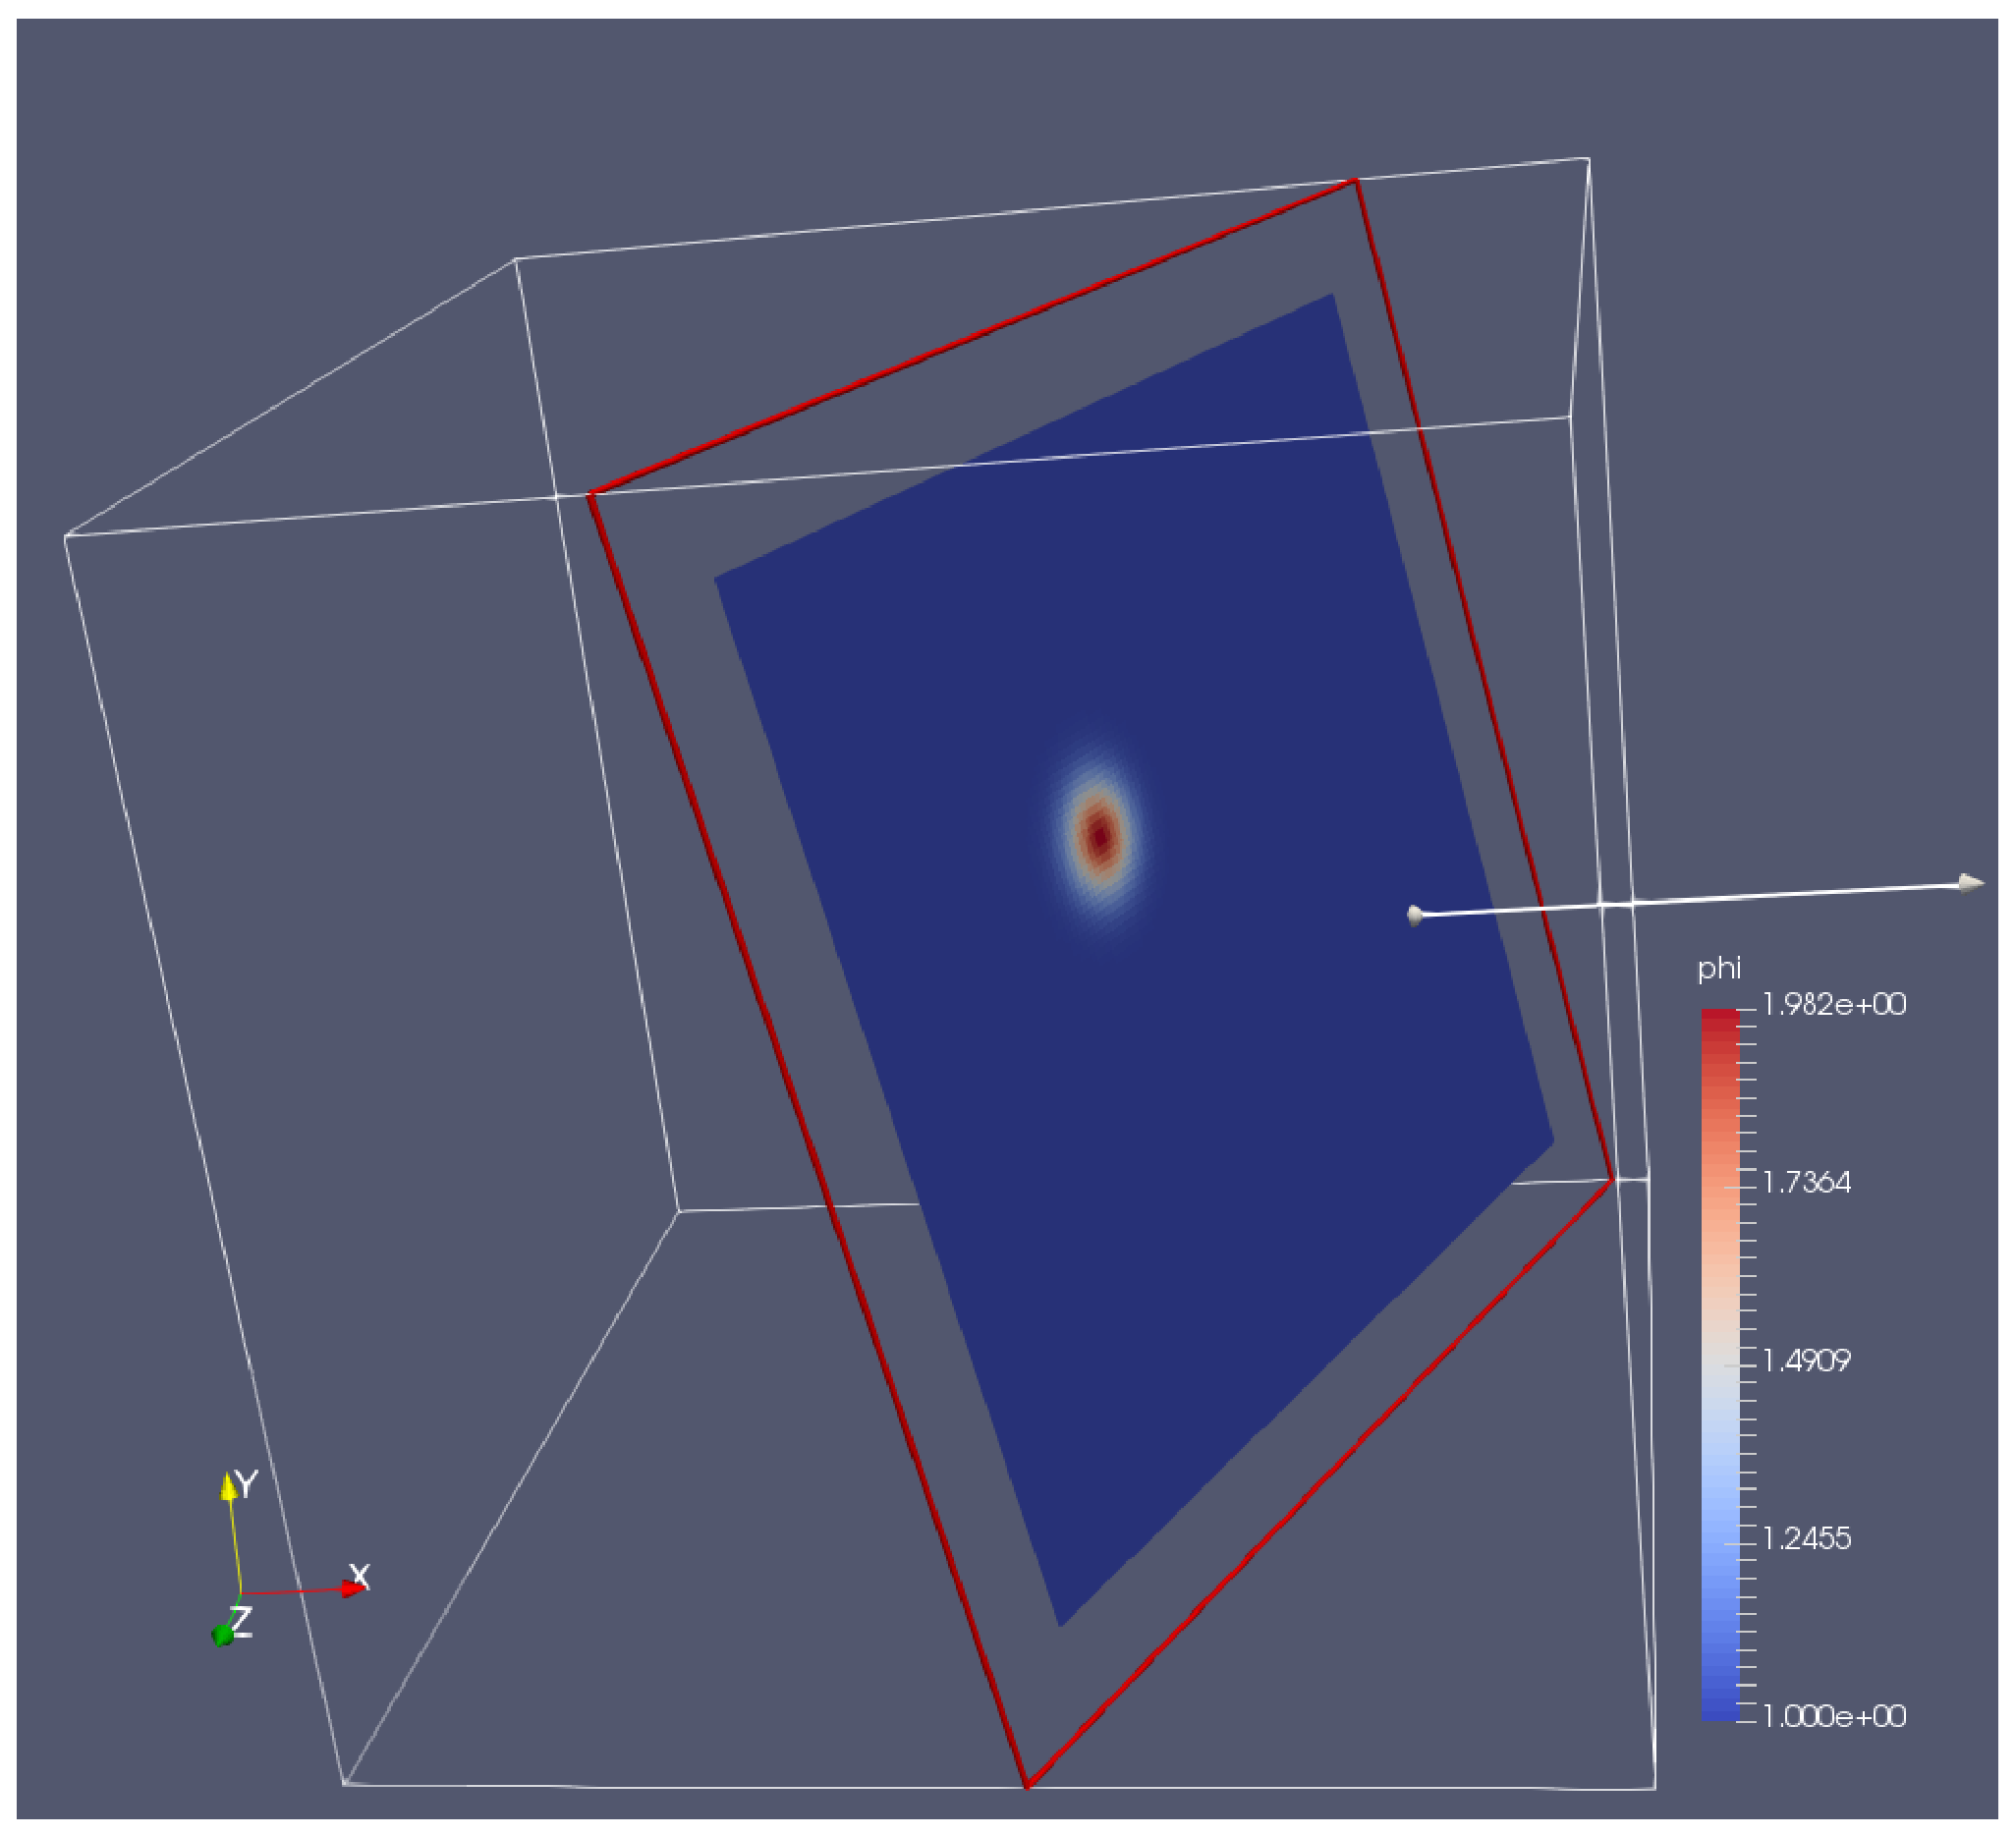
\includegraphics[width=3.1in]{./Visualization/ParaView}
\caption{Plotfile image generated with \paraview}
\label{fig:ParaView}
\end{figure}

To visualize particles (for example, you could run the {\tt ShortRangeParticles} example:
\begin{enumerate}
\item First, we have to convert the \amrex\ particle data to a format \paraview\ can read.
      In the run directory, there will be a sequence of particle files ({\tt particles00000},
      {\tt particles00001}, $\cdots$, {\tt particles01000}).
\item Run the script,
      {\tt amrex/Tools/Py\_util/amrex\_particles\_to\_vtp/amrex\_particles\_to\_vtp.py}
      as follows, e.g.,
      {\tt python amrex\_particles\_to\_vtp.py 0 1000 particles}.  You will generate
      a sequence of {\tt .vtp} files.
\item Run \paraview v5.4.0, and select ``File'' $\rightarrow$ ``Open''.  You will see
      a combined ``particles..vtp'' file grouping the files.  Select that and click OK.
\item Click ``Apply'' and under ``Representation'' select ``Point Gaussian''.
\item Change the Gaussian Radius if you like.  You can scroll through the frames with the
      VCR-like controls at the top, as shown in Figure \ref{fig:ParaView_particles}.
\end{enumerate}


\begin{figure}[tb]
\centering
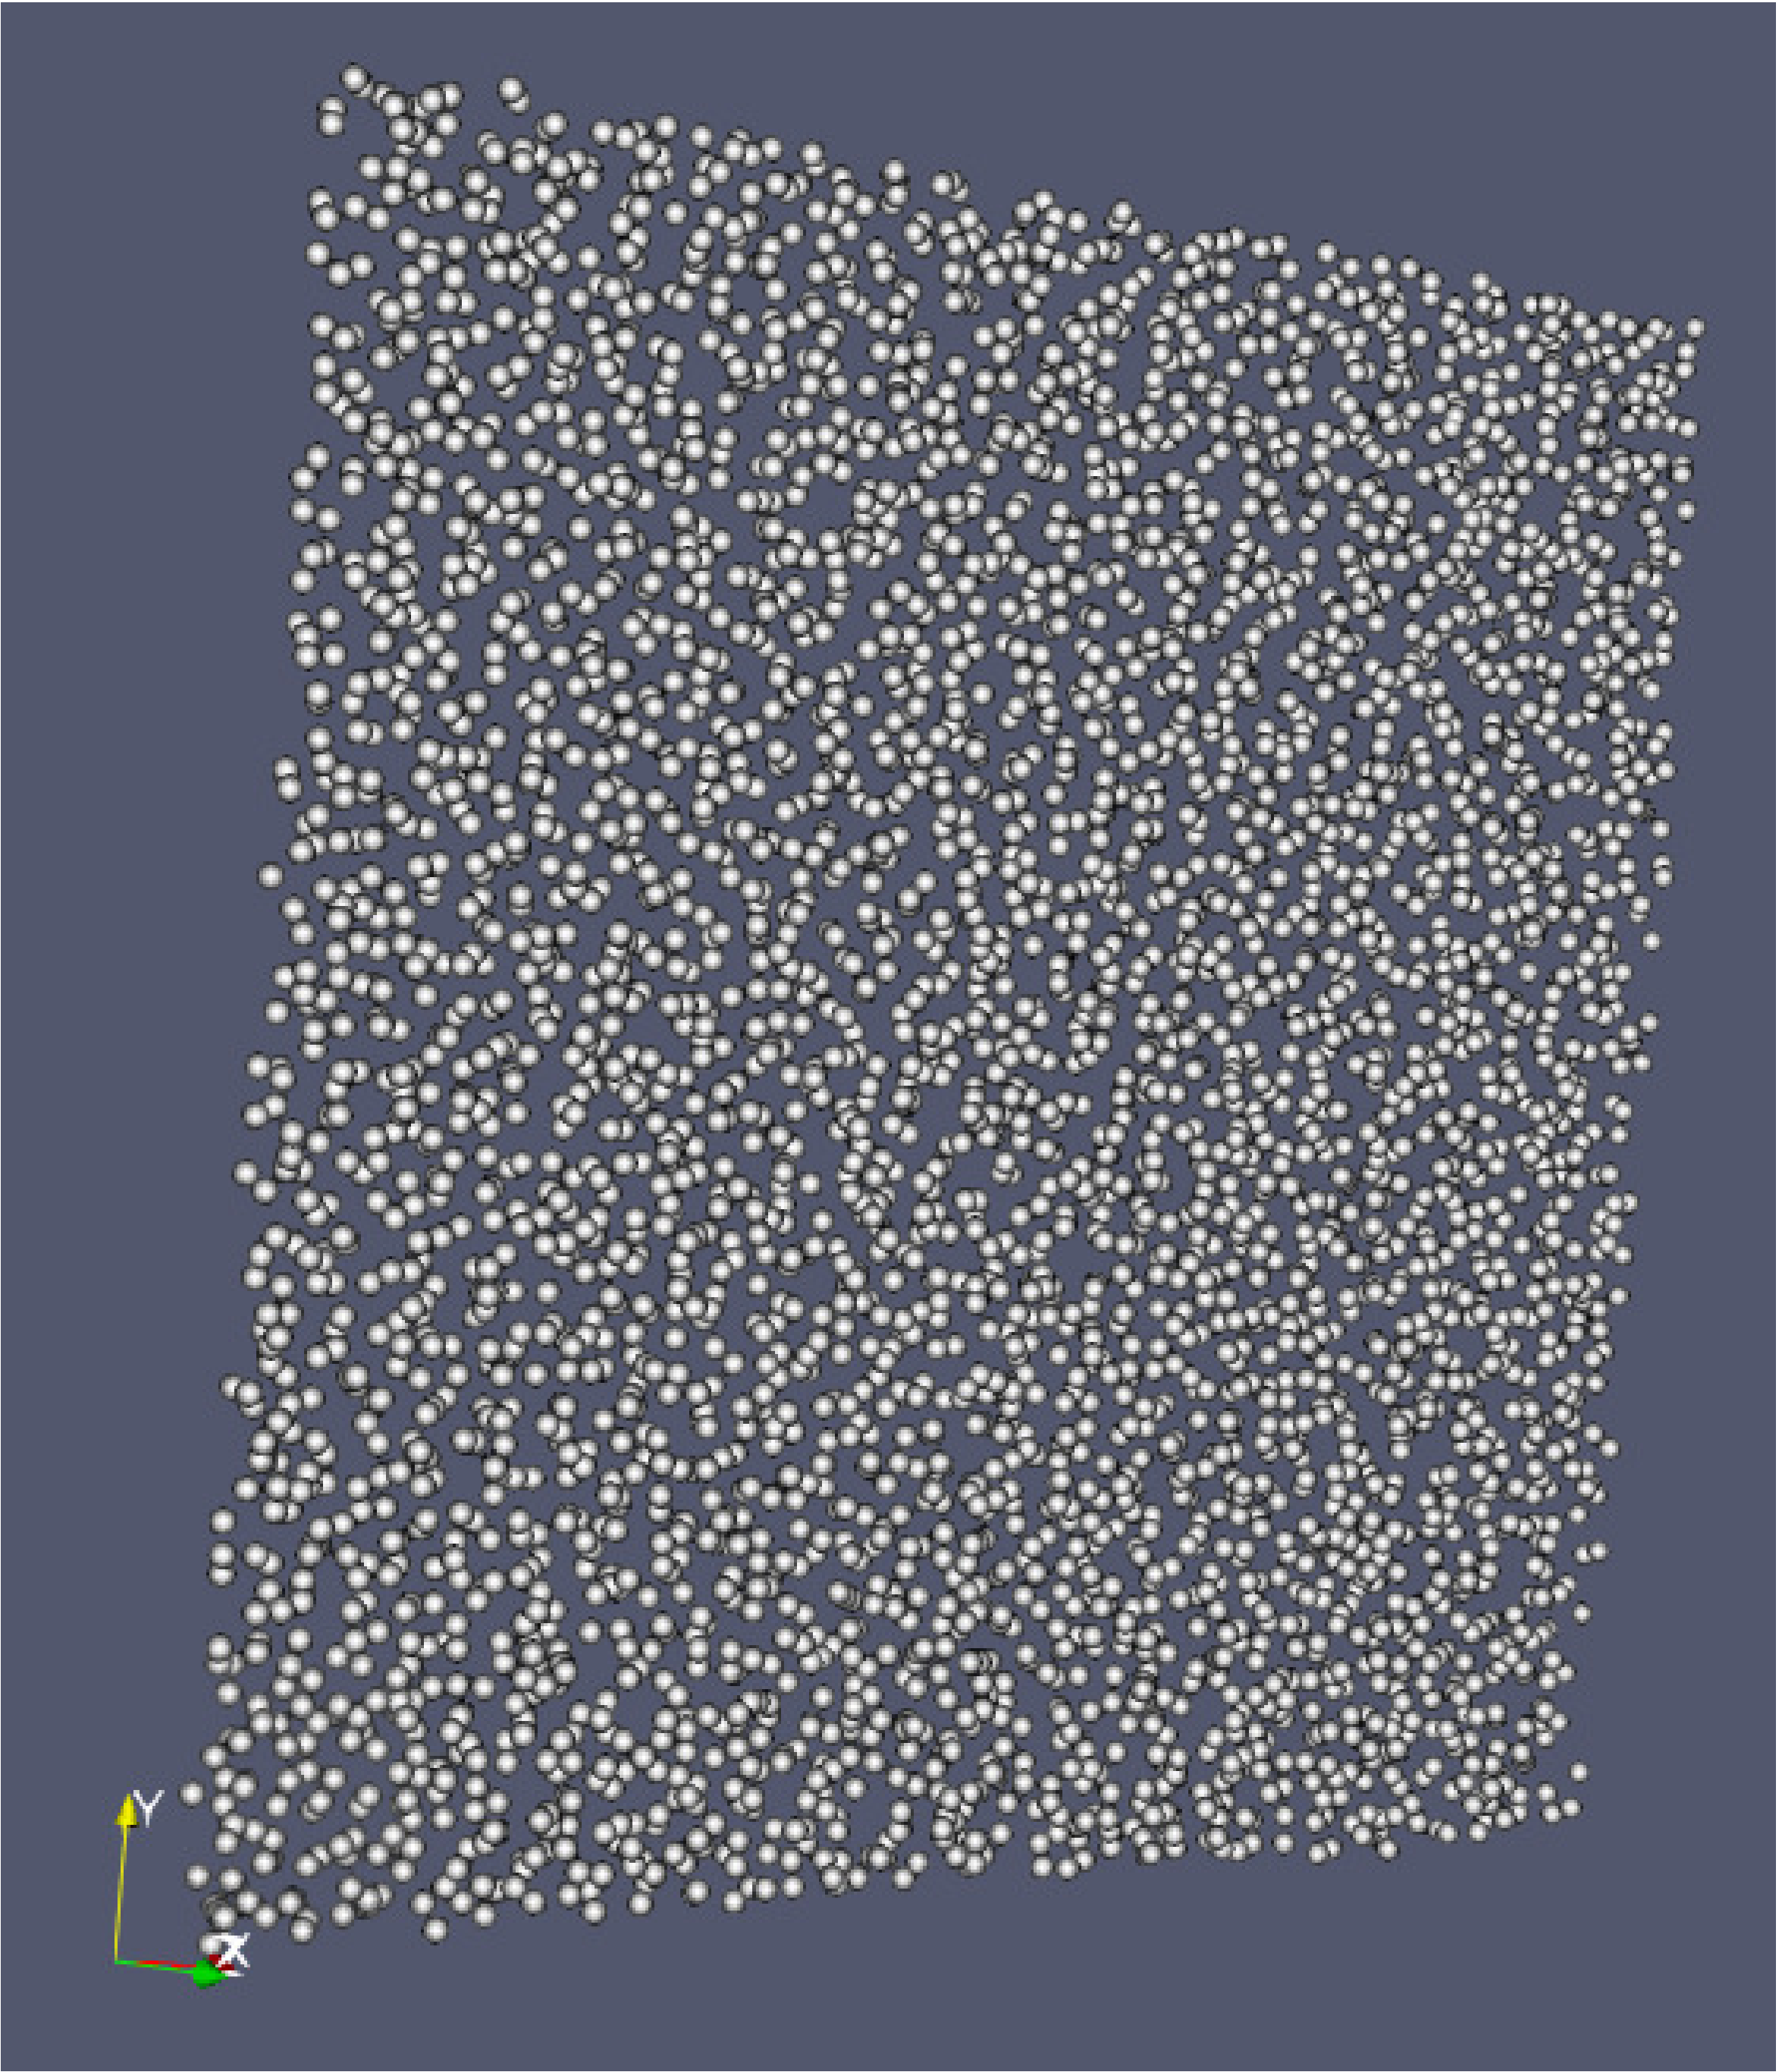
\includegraphics[width=3.1in]{./Visualization/ParaView_particles}
\caption{Particle image generated with \paraview}
\label{fig:ParaView_particles}
\end{figure}

\section{\yt}

\yt, an open source Python package available at \url{http://yt-project.org/},
can be used for analyzing and visualizing mesh and particle data generated by
\amrex\ codes.  Some of the \amrex\ developers are also \yt\ project members.
Below we describe how to use \yt\ on both a local workstation, as well as at
the NERSC HPC facility for high-throughput visualization of large data sets.

\subsection{Using \yt\ on a local workstation}

Running \yt\ on a local system generally provides good interactivity, but
limited performance. Consequently, this configuration is best when doing
exploratory visualization (e.g., experimenting with camera angles, lighting,
and color schemes) of small data sets.

To use \yt\ on an \amrex\ plot file, first start a Jupyter notebook or an IPython kernel, and import the \texttt{yt} module:

\begin{lstlisting}[language=python,breaklines=true]
In [1]: import yt

In [2]: print(yt.__version__)
3.4-dev
\end{lstlisting}

Next, load a plot file; in this example we use a plot file from the Nyx cosmology application:

\begin{lstlisting}[language=python,breaklines=true]
In [3]: ds = yt.load("plt00401")
yt : [INFO     ] 2017-05-23 10:03:56,182 Parameters: current_time              = 0.00605694344696544
yt : [INFO     ] 2017-05-23 10:03:56,182 Parameters: domain_dimensions         = [128 128 128]
yt : [INFO     ] 2017-05-23 10:03:56,182 Parameters: domain_left_edge          = [ 0.  0.  0.]
yt : [INFO     ] 2017-05-23 10:03:56,183 Parameters: domain_right_edge         = [ 14.24501  14.24501  14.24501]

In [4]: ds.field_list
Out[4]:
[('DM', 'particle_mass'),
 ('DM', 'particle_position_x'),
 ('DM', 'particle_position_y'),
 ('DM', 'particle_position_z'),
 ('DM', 'particle_velocity_x'),
 ('DM', 'particle_velocity_y'),
 ('DM', 'particle_velocity_z'),
 ('all', 'particle_mass'),
 ('all', 'particle_position_x'),
 ('all', 'particle_position_y'),
 ('all', 'particle_position_z'),
 ('all', 'particle_velocity_x'),
 ('all', 'particle_velocity_y'),
 ('all', 'particle_velocity_z'),
 ('boxlib', 'density'),
 ('boxlib', 'particle_mass_density')]
\end{lstlisting}

From here one can make slice plots, 3-D volume renderings, etc. An example of
the slice plot feature is shown below:

\begin{lstlisting}[language=python,breaklines=true]
In [9]: slc = yt.SlicePlot(ds, "z", "density")
yt : [INFO     ] 2017-05-23 10:08:25,358 xlim = 0.000000 14.245010
yt : [INFO     ] 2017-05-23 10:08:25,358 ylim = 0.000000 14.245010
yt : [INFO     ] 2017-05-23 10:08:25,359 xlim = 0.000000 14.245010
yt : [INFO     ] 2017-05-23 10:08:25,359 ylim = 0.000000 14.245010

In [10]: slc.show()

In [11]: slc.save()
yt : [INFO     ] 2017-05-23 10:08:34,021 Saving plot plt00401_Slice_z_density.png
Out[11]: ['plt00401_Slice_z_density.png']
\end{lstlisting}

The resulting image is Figure~\ref{fig:yt_Nyx_slice_plot}. One can also make
volume renderings with \yt; an example is show below:

\begin{figure}
  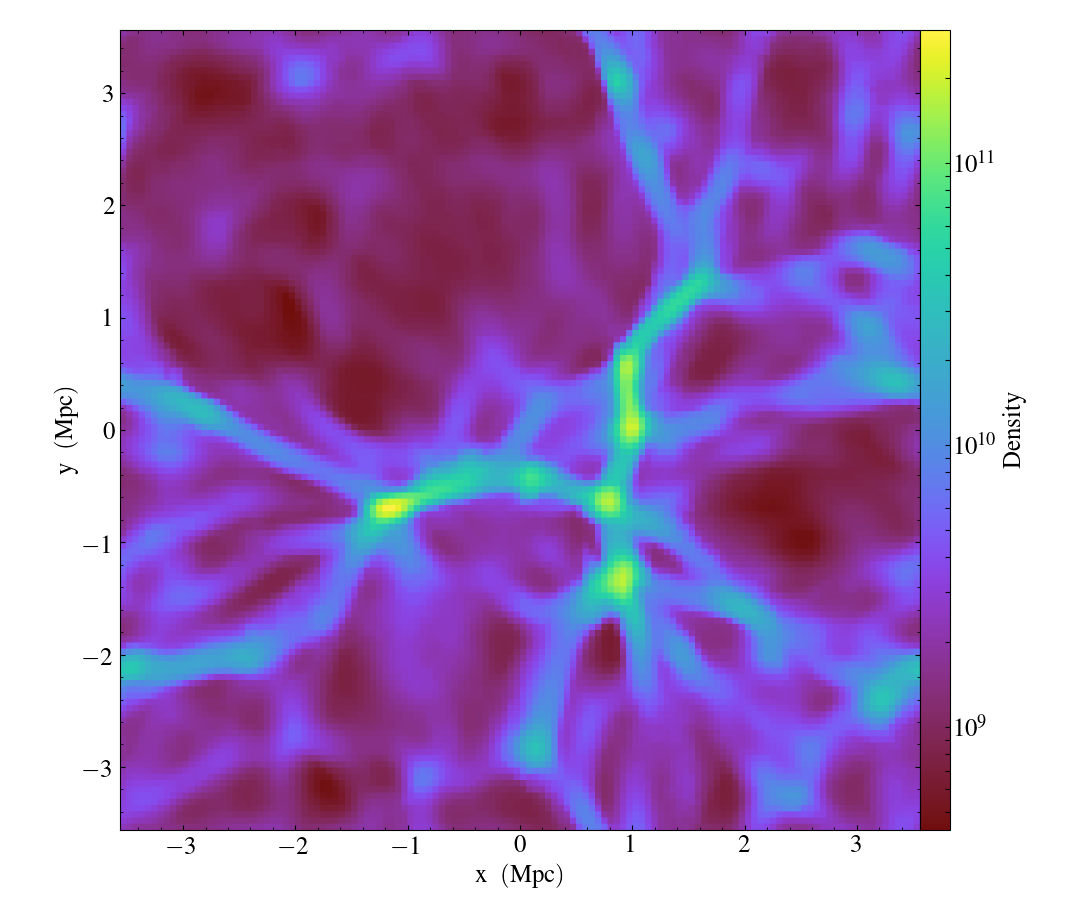
\includegraphics[scale=0.5]{./Visualization/yt_Nyx_density_slice.png}
  \caption{Slice plot of $128^3$ Nyx simulation using \yt.}
  \label{fig:yt_Nyx_slice_plot}
\end{figure}

\begin{lstlisting}[language=python,breaklines=true]
In [12]: sc = yt.create_scene(ds, field="density", lens_type="perspective")

In [13]: source = sc[0]

In [14]: source.tfh.set_bounds((1e8, 1e15))

In [15]: source.tfh.set_log(True)

In [16]: source.tfh.grey_opacity = True

In [17]: sc.show()
<Scene Object>:
Sources:
    source_00: <Volume Source>:YTRegion (plt00401): , center=[  1.09888770e+25   1.09888770e+25   1.09888770e+25] cm, left_edge=[ 0.  0.  0.] cm, right_edge=[  2.19777540e+25   2.19777540e+25   2.19777540e+25] cm transfer_function:None
Camera:
    <Camera Object>:
	position:[ 14.24501  14.24501  14.24501] code_length
	focus:[ 7.122505  7.122505  7.122505] code_length
	north_vector:[ 0.81649658 -0.40824829 -0.40824829]
	width:[ 21.367515  21.367515  21.367515] code_length
	light:None
	resolution:(512, 512)
Lens: <Lens Object>:
	lens_type:perspective
	viewpoint:[ 0.95423473  0.95423473  0.95423473] code_length

In [19]: sc.save()
yt : [INFO     ] 2017-05-23 10:15:07,825 Rendering scene (Can take a while).
yt : [INFO     ] 2017-05-23 10:15:07,825 Creating volume
yt : [INFO     ] 2017-05-23 10:15:07,996 Creating transfer function
yt : [INFO     ] 2017-05-23 10:15:07,997 Calculating data bounds. This may take a while.  Set the TranferFunctionHelper.bounds to avoid this.
yt : [INFO     ] 2017-05-23 10:15:16,471 Saving render plt00401_Render_density.png
\end{lstlisting}

The output of this is Figure~\ref{fig:yt_Nyx_vol_rend}.

\begin{figure}
  
\includegraphics[scale=1.0]{./Visualization/yt_Nyx_density_vol_rend.png}
  \caption{Volume rendering of $128^3$ Nyx simulation using \yt. This
           corresponds to the same plot file used to generate the slice plot in
           Figure~\ref{fig:yt_Nyx_slice_plot}.}
  \label{fig:yt_Nyx_vol_rend}
\end{figure}

\subsection{Using \yt\ at NERSC (\emph{under development})}

Becase \yt\ is Python-based, it is portable and can be used in many software
environments. Here we focus on \yt's capabilities at NERSC, which provides
resources for performing both interactive and batch queue-based visualization
and analysis of \amrex\ data. Coupled with \yt's MPI and OpenMP parallelization
capabilities, this can enable high-throughput visualization and analysis
workflows.

\subsubsection{Interactive \yt\ with Jupyter notebooks}

Unlike \visit\ (\S\ref{sec:visit}), \yt\ has no client-server interface. Such
an interface is often crucial when one has large data sets generated on a
remote system, but wishes to visualize the data on a local workstation. Both
copying the data between the two systems, as well as visualizing the data
itself on a workstation, can be prohibitively slow.

Fortunately, NERSC has implemented several resources which allow one to
interact with \yt\ remotely, emulating a client-server model. In particular,
NERSC now hosts Jupyter notebooks which run IPython kernels on the Cori system;
this provides users access to the \texttt{\$HOME}, \texttt{/project}, and
\texttt{\$SCRATCH} file systems from a web browser-based Jupyter notebook.
\emph{\textbf{Please note that Jupyter hosting at NERSC is still under
development, and the environment may change without notice.}}

NERSC also provides Anaconda Python, which allows users to create their own
customizable Python environments. It is recommended to install \yt\ in such an
environment. One can do so with the following example:

\begin{lstlisting}
user@cori10:~> module load python/3.5-anaconda
user@cori10:~> conda create -p $HOME/yt-conda numpy
user@cori10:~> source activate $HOME/yt-conda
(/global/homes/u/user/yt-conda/) user@cori10:~> pip install yt
\end{lstlisting}

More information about Anaconda Python at NERSC is here:
\url{http://www.nersc.gov/users/data-analytics/data-analytics/python/anaconda-python/}.

One can then configure this Anaconda environment to run in a Jupyter notebook
hosted on the Cori system. Currently this is available in two places: on
\url{https://ipython.nersc.gov}, and on \url{https://jupyter-dev.nersc.gov}.
The latter likely reflects what the stable, production environment for Jupyter
notebooks will look like at NERSC, but it is still under development and
subject to change. To load this custom Python kernel in a Jupyter notebook,
follow the instructions at this URL under the ``Custom Kernels'' heading:
\url{http://www.nersc.gov/users/data-analytics/data-analytics/web-applications-for-data-analytics}.
After writing the appropriate \texttt{kernel.json} file, the custom kernel will
appear as an available Jupyter notebook. Then one can interactively visualize
\amrex\ plot files in the web browser.\footnote{It is convenient to use the
magic command \texttt{\%matplotlib inline} in order to render matplotlib
figures in the same browser window as the notebook, as opposed to displaying it
as a new window.}

\subsubsection{Parallel \yt}

Besides the benefit of no longer needing to move data back and forth between
NERSC and one's local workstation to do visualization and analysis, an
additional feature of \yt\ which takes advantage of the computational resources
at NERSC is its parallelization capabilities. \yt\ supports both MPI- and
OpenMP-based parallelization of various tasks, which are discussed here:
\url{http://yt-project.org/doc/analyzing/parallel_computation.html}.

Configuring \yt\ for MPI parallelization at NERSC is a more complex task than
discussed on the official \yt\ documentation; the command \texttt{pip install
mpi4py} is not sufficient. Rather, one must compile \texttt{mpi4py} from source
using the Cray compiler wrappers \texttt{cc}, \texttt{CC}, and \texttt{ftn} on
Cori. Instructions for compiling \texttt{mpi4py} at NERSC are provided here:
\url{http://www.nersc.gov/users/data-analytics/data-analytics/python/anaconda-python/#toc-anchor-3}.
After \texttt{mpi4py} has been compiled, one can use the regular Python
interpreter in the Anaconda environment as normal; when executing \yt\
operations which support MPI parallelization, the multiple MPI processes will
spawn automatically.

Although several components of \yt\ support MPI parallelization, a few are particularly useful:
\begin{itemize}
  \item \textbf{Time series analysis.} Often one runs a simulation for many
time steps and periodically writes plot files to disk for visualization and
post-processing. \yt\ supports parallelization over time series data via the
\texttt{DatasetSeries} object. \yt\ can iterate over a \texttt{DatasetSeries}
in parallel, with different MPI processes operating on different elements of
the series. This page provides more documentation:
\url{http://yt-project.org/doc/analyzing/time_series_analysis.html#time-series-analysis}.

  \item \textbf{Volume rendering}. \yt\ implements spatial decomposition among
MPI processes for volume rendering procedures, which can be computationally
expensive. Note that \yt\ also implements OpenMP parallelization in volume
rendering, and so one can execute volume rendering with a hybrid MPI+OpenMP
approach. See this URL for more details:
\url{http://yt-project.org/doc/visualizing/volume_rendering.html?highlight=openmp#openmp-parallelization}.

  \item \textbf{Generic parallelization over multiple objects.} Sometimes one
wishes to loop over a series which is not a \texttt{DatasetSeries}, e.g.,
performing translational or rotational operations on a camera to make a volume
rendering in which the field of view moves through the simulation. In this
case, one is applying a set of operations on a single object (a single plot
file), rather than over a time series of data. For this workflow, \yt\ provides
the \texttt{parallel\_objects()} function. See this URL for more details:
\url{http://yt-project.org/doc/analyzing/parallel_computation.html#parallelizing-over-multiple-objects}.

An example of MPI parallelization in \yt\ is shown below, where one animates a
time series of plot files from an IAMR simulation while revolving the camera
such that it completes two full revolutions over the span of the animation:

\begin{lstlisting}[language=python,breaklines=true]
import yt
import glob
import numpy as np

yt.enable_parallelism()

base_dir1 = '/global/cscratch1/sd/user/Nyx_run_p1'
base_dir2 = '/global/cscratch1/sd/user/Nyx_run_p2'
base_dir3 = '/global/cscratch1/sd/user/Nyx_run_p3'

glob1 = glob.glob(base_dir1 + '/plt*')
glob2 = glob.glob(base_dir2 + '/plt*')
glob3 = glob.glob(base_dir3 + '/plt*')

files = sorted(glob1 + glob2 + glob3)

ts = yt.DatasetSeries(files, parallel=True)

frame = 0
num_frames = len(ts)
num_revol = 2

slices = np.arange(len(ts))

for i in yt.parallel_objects(slices):
    sc = yt.create_scene(ts[i], lens_type='perspective', field='z_velocity')

    source = sc[0]
    source.tfh.set_bounds((1e-2, 9e+0))
    source.tfh.set_log(False)
    source.tfh.grey_opacity = False

    cam = sc.camera

    cam.rotate(num_revol*(2.0*np.pi)*(i/num_frames),
               rot_center=np.array([0.0, 0.0, 0.0]))

    sc.save(sigma_clip=5.0)
\end{lstlisting}

When executed on 4 CPUs on a Haswell node of Cori, the output looks like the following:

\begin{lstlisting}[breaklines=true]
user@nid00009:~/yt_vis/> srun -n 4 -c 2 --cpu_bind=cores python make_yt_movie.py
yt : [INFO     ] 2017-05-23 16:51:33,565 Global parallel computation enabled: 0 / 4
yt : [INFO     ] 2017-05-23 16:51:33,565 Global parallel computation enabled: 2 / 4
yt : [INFO     ] 2017-05-23 16:51:33,566 Global parallel computation enabled: 1 / 4
yt : [INFO     ] 2017-05-23 16:51:33,566 Global parallel computation enabled: 3 / 4
P003 yt : [INFO     ] 2017-05-23 16:51:33,957 Parameters: current_time              = 0.103169376949795
P003 yt : [INFO     ] 2017-05-23 16:51:33,957 Parameters: domain_dimensions         = [128 128 128]
P003 yt : [INFO     ] 2017-05-23 16:51:33,957 Parameters: domain_left_edge          = [ 0.  0.  0.]
P003 yt : [INFO     ] 2017-05-23 16:51:33,958 Parameters: domain_right_edge         = [ 6.28318531  6.28318531  6.28318531]
P000 yt : [INFO     ] 2017-05-23 16:51:33,969 Parameters: current_time              = 0.0
P000 yt : [INFO     ] 2017-05-23 16:51:33,969 Parameters: domain_dimensions         = [128 128 128]
P002 yt : [INFO     ] 2017-05-23 16:51:33,969 Parameters: current_time              = 0.0687808060674485
P000 yt : [INFO     ] 2017-05-23 16:51:33,969 Parameters: domain_left_edge          = [ 0.  0.  0.]
P002 yt : [INFO     ] 2017-05-23 16:51:33,969 Parameters: domain_dimensions         = [128 128 128]
P000 yt : [INFO     ] 2017-05-23 16:51:33,970 Parameters: domain_right_edge         = [ 6.28318531  6.28318531  6.28318531]
P002 yt : [INFO     ] 2017-05-23 16:51:33,970 Parameters: domain_left_edge          = [ 0.  0.  0.]
P002 yt : [INFO     ] 2017-05-23 16:51:33,970 Parameters: domain_right_edge         = [ 6.28318531  6.28318531  6.28318531]
P001 yt : [INFO     ] 2017-05-23 16:51:33,973 Parameters: current_time              = 0.0343922351851018
P001 yt : [INFO     ] 2017-05-23 16:51:33,973 Parameters: domain_dimensions         = [128 128 128]
P001 yt : [INFO     ] 2017-05-23 16:51:33,974 Parameters: domain_left_edge          = [ 0.  0.  0.]
P001 yt : [INFO     ] 2017-05-23 16:51:33,974 Parameters: domain_right_edge         = [ 6.28318531  6.28318531  6.28318531]
P000 yt : [INFO     ] 2017-05-23 16:51:34,589 Rendering scene (Can take a while).
P000 yt : [INFO     ] 2017-05-23 16:51:34,590 Creating volume
P003 yt : [INFO     ] 2017-05-23 16:51:34,592 Rendering scene (Can take a while).
P002 yt : [INFO     ] 2017-05-23 16:51:34,592 Rendering scene (Can take a while).
P003 yt : [INFO     ] 2017-05-23 16:51:34,593 Creating volume
P002 yt : [INFO     ] 2017-05-23 16:51:34,593 Creating volume
P001 yt : [INFO     ] 2017-05-23 16:51:34,606 Rendering scene (Can take a while).
P001 yt : [INFO     ] 2017-05-23 16:51:34,607 Creating volume
\end{lstlisting}

Because the \texttt{parallel\_objects()} function transforms the loop into a
data-parallel problem, this procedure strong scales nearly perfectly to an
arbitrarily large number of MPI processes, allowing for rapid rendering of
large time series of data.

\end{itemize}
